\subsection{Visual C++ ビルド ツールをインストールする}

Rust には、Visual Studio 2013 以降の Microsoft C++ ビルド ツールが必要です。 Rust をインストールするには、事前にこれらのビルド ツールがインストールされている必要があります。

ビルド ツールがインストールされていない場合は、次の手順に従います。


\begin{enumerate}
\item Microsoft Visual Studio Code のダウンロード ページにアクセスします。

\item $[$Build Tools のダウンロード] を選択します。

\item ダウンロードが完了したら、インストーラー ファイルを実行します。 Visual Studio インストーラー ウィンドウが開きます。

\item ポップアップ ダイアログで、[はい] を選択します。 次のポップアップ ダイアログで、[続行] を選択します。

\item インストーラー ウィンドウの [デスクトップとモバイル] で、左側にある [C++ Build Tools] オプションのチェックボックスをオンにします。

\item 右側の [インストールの詳細] ウィンドウで、次のオプションが選択されていることを確認します。
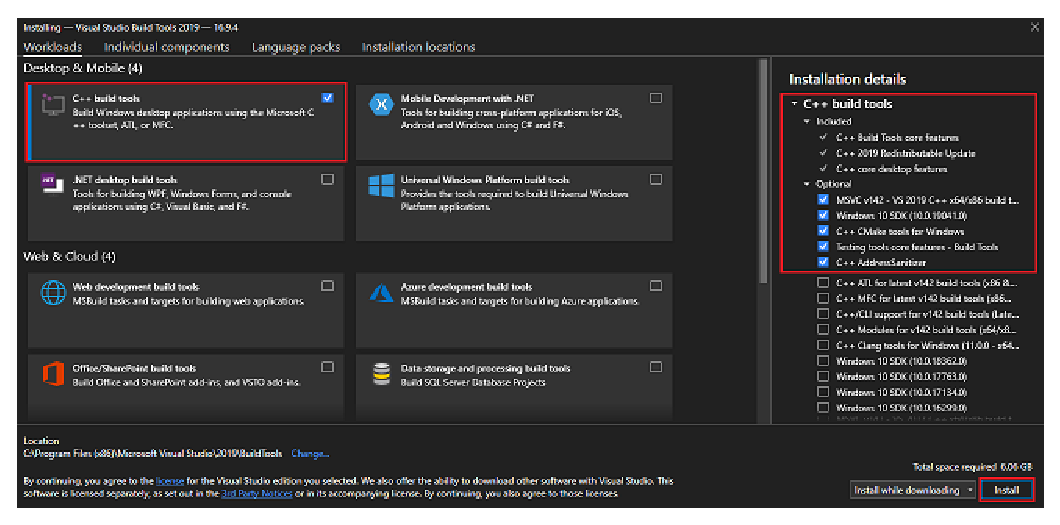
\includegraphics[width=14cm]{install-visual-cpp-build-tools.eps}

\item 右下にある [インストール] を選択します。
\end{enumerate}

インストールが完了したら、Rust のインストールを続行できます。
